\documentclass[10pt]{article}

\usepackage[margin=0.6in]{geometry}
\usepackage{enumitem}
\usepackage{titlesec}
\usepackage{xcolor}
\usepackage{graphicx}
\usepackage{hyperref}
\definecolor{linkblue}{HTML}{0B5FA5}
\hypersetup{colorlinks=true, urlcolor=linkblue, linkcolor=linkblue, citecolor=linkblue}
\usepackage{parskip}

\titleformat{\section}{\large\bfseries}{}{0em}{}[{\vspace{-5pt}\rule{\linewidth}{0.6pt}}]
\titlespacing{\section}{0pt}{6pt}{3pt}
\setlist[itemize,1]{leftmargin=1.2em, itemsep=1pt, topsep=1pt}
\setlist[itemize,2]{leftmargin=0.75em, labelsep=0.28em, itemsep=0.6pt, topsep=1pt,
                    label=\raisebox{0.2ex}{\rule{0.25em}{0.25em}}}
\pagestyle{empty}
\setlength{\parskip}{2pt}
\newcommand{\me}{\textbf{M.\ Islam}}

% Sub-project block inside an experience entry
\newenvironment{subprojects}
  {\begin{itemize}[label={}, leftmargin=0.9em, itemsep=3pt, topsep=2pt]}
  {\end{itemize}}

\begin{document}

%========================= HEADER =========================
\noindent
\begin{minipage}[c]{0.11\textwidth}
    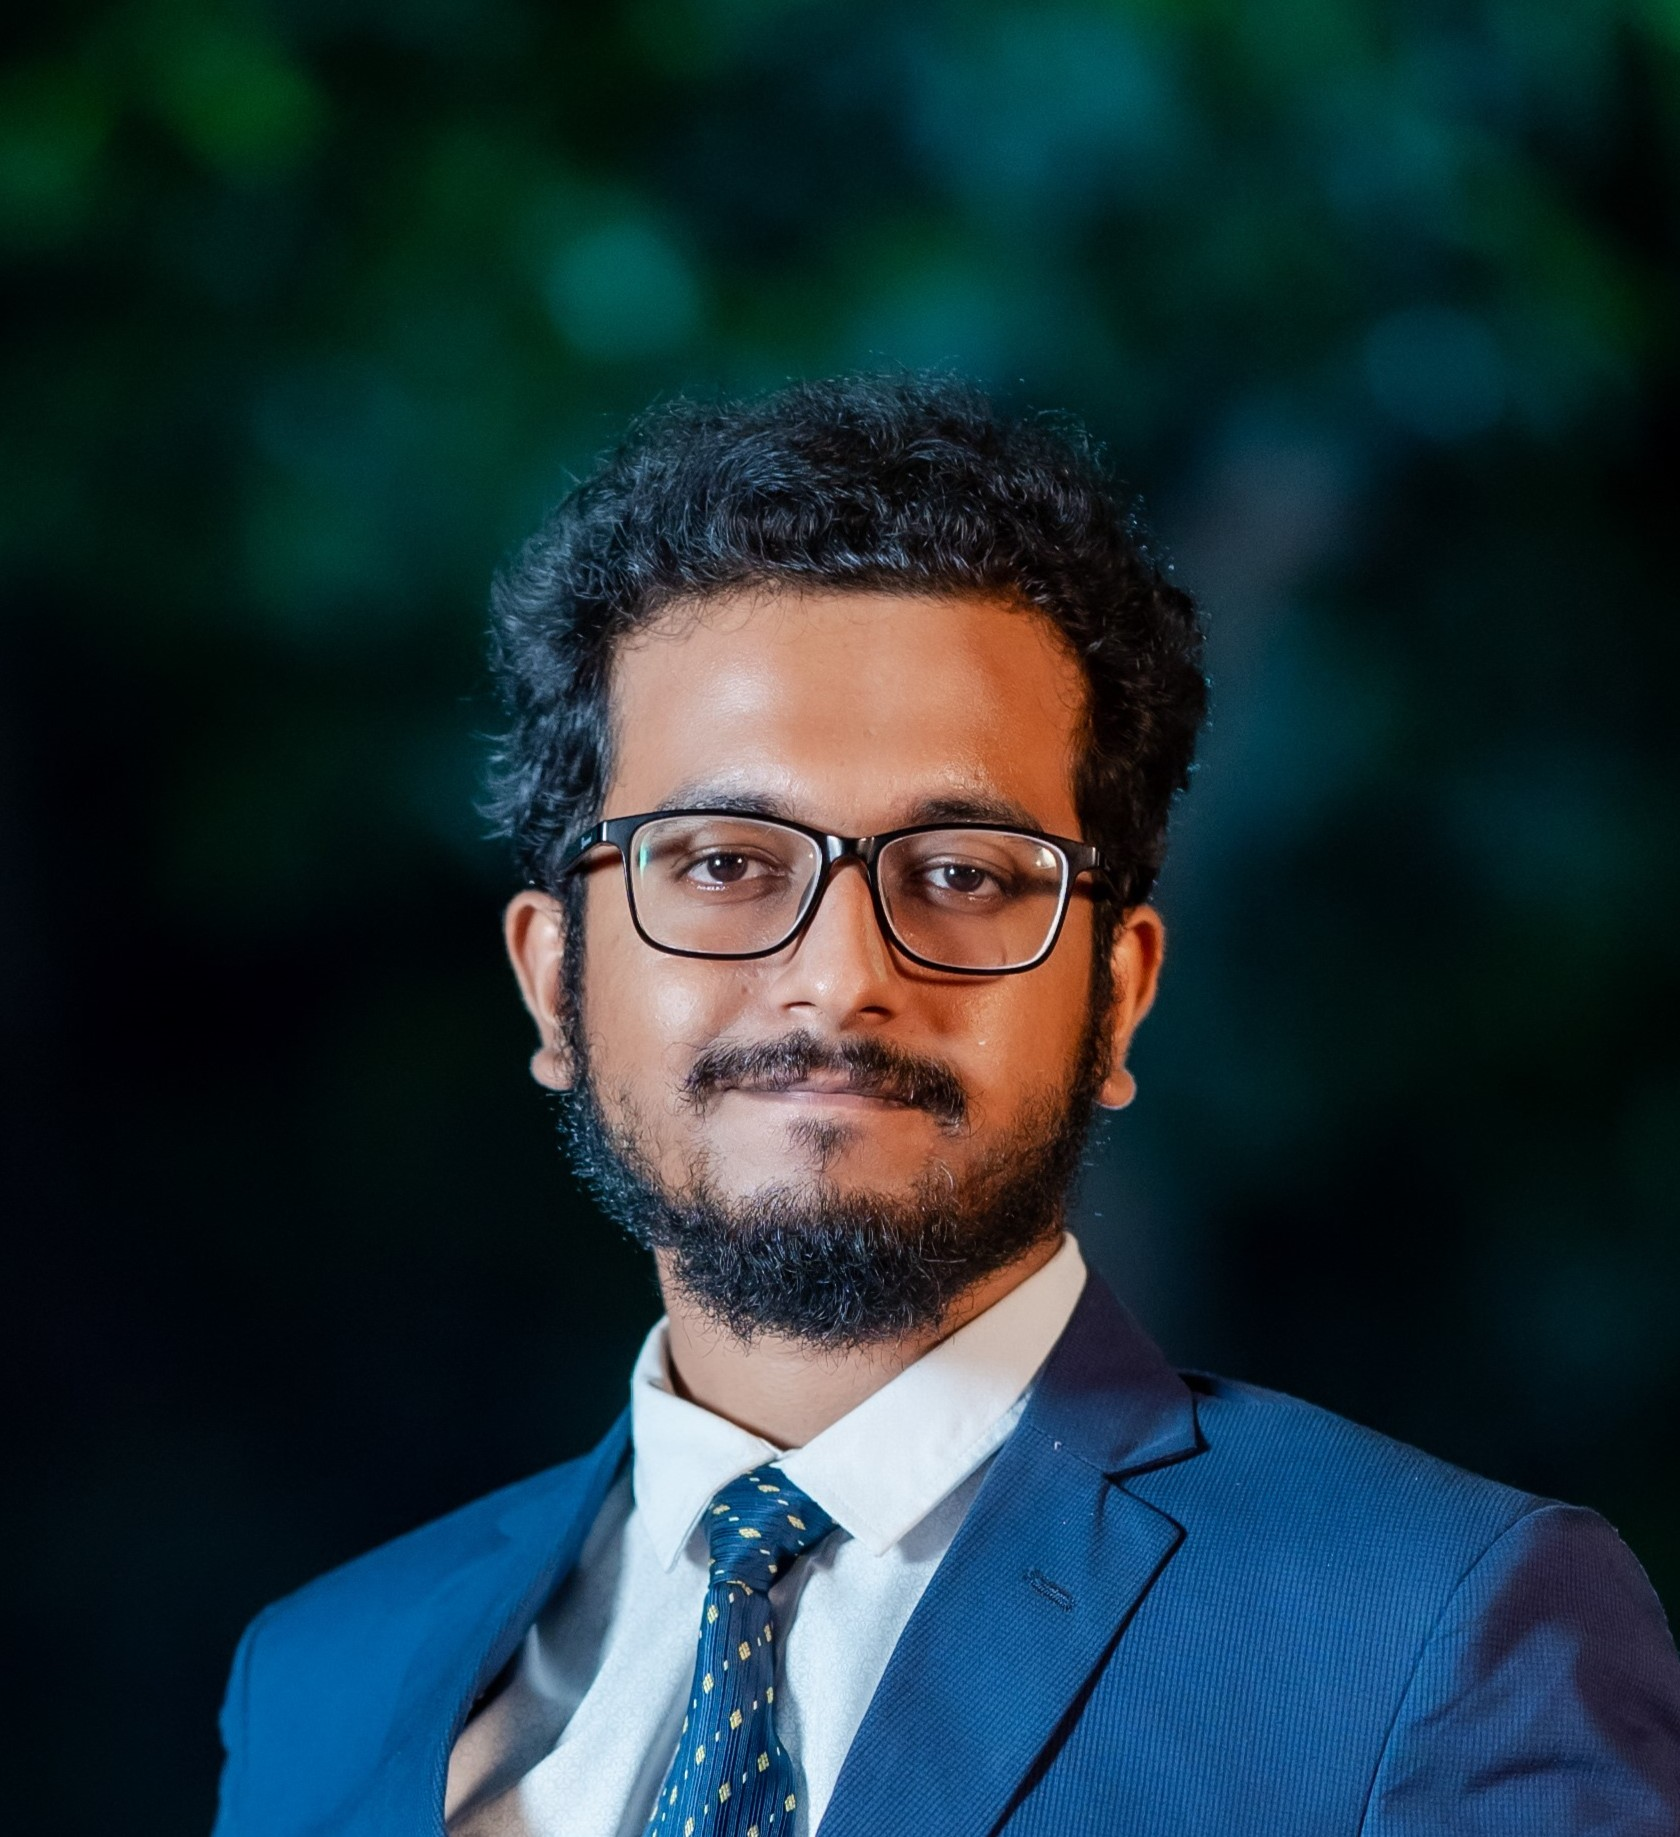
\includegraphics[width=\linewidth]{photo.jpg}
\end{minipage}%
\begin{minipage}[c]{0.78\textwidth}
    \centering
    {\LARGE\bfseries Mainul Islam}\\[3pt]
    \href{mailto:mainulislam@iut-dhaka.edu}{mainulislam@iut-dhaka.edu} \;\textbar\;
    \href{https://scholar.google.com/citations?user=mHfGHugAAAAJ\&hl=en}{Google Scholar} \;\textbar\;
    \href{https://www.linkedin.com/in/mainul-islam-254071205/}{LinkedIn} \;\textbar\;
    \href{https://mainul-islam-07.github.io/mainulislam.github.io/}{Portfolio} \;\textbar\;
    \href{https://www.youtube.com/@mainulislamefan}{YouTube}
\end{minipage}%
\begin{minipage}[c]{0.11\textwidth}
    \hspace{0pt}
\end{minipage}

%========================= PROFESSIONAL EXPERIENCE =========================
\section*{Professional Experience}

\textbf{R\&D Engineer (Robotics \& Embedded Systems)} ---
\href{https://cyberneticsbd.com/}{Cybernetics Hi-Tech Solutions}
\hfill Oct 2024 -- Present

\vspace{1pt}
Embedded and robotic systems from requirements through field commissioning --- control
electronics, bare-metal firmware, networking, and operator interfaces. Selected deliveries:

\begin{subprojects}

    \item \textbf{\href{https://www.youtube.com/watch?v=v_SOAQoPP6Q}{Man-Transportable EOD Robot
    (Jontro Soinik 2.0)}}
    \begin{itemize}
        \item Wrote the bare-metal C firmware for two STM32F103 (ARM Cortex-M3, HAL) nodes forming
        a redundant serial-over-Ethernet link: UART DMA with idle-line detection for variable-length
        binary frames, a WIZnet W5500 TCP/IP controller over SPI, and UDP transport.
        \item Structured interrupt handling as a deferred-ISR pattern (an EXTI line latches W5500
        socket events for main-loop service), with a TIM watchdog that fails over to the wireless
        link via GPIO relay lines when the wired stream stops.
        \item Developed the object-oriented motion-control library for eleven servo drives on two
        independent 1\,Mbit/s CAN buses, implementing CANopen (CiA-402) so that each joint can be
        commanded by position, speed, or torque.
        \item Contributed a closed-form solution to the arm's inverse kinematics, integrated with
        MoveIt\,2 for collision checking.
        \item Developed the operator application: low-latency video, a UDP/JSON telemetry dashboard,
        and a 3D on-screen model of the robot's posture.
    \end{itemize}

    \item \textbf{\href{https://youtu.be/TkmOu6lCBTw?si=8KOdXk-vVMPzP4vm}{Autonomous Guided Vehicle
    --- CYBERFLEET}}
    \begin{itemize}
        \item Designed the complete ROS\,2 system integration for a three-vehicle warehouse robot
        fleet --- localisation, routing, path following, and coordination.
        \item Implemented an extended Kalman filter fusing wheel-encoder motion with intermittent
        camera sightings of fixed floor markers, plus calibration and per-marker pose estimation.
        \item Contributed time-indexed route planning that prevents collisions and deadlocks, and
        LiDAR-based obstacle detection.
    \end{itemize}

    \item \textbf{\href{https://www.youtube.com/watch?v=tsnFWpL0otE&list=PL83KI7SnKe-WVnVozQg_rh70uutLMiiNe&index=3}{Toll-Booth
    Automation}}
    \begin{itemize}
        \item Developed the lane-controller firmware in embedded C on an STM32, structured as a
        table-driven state machine.
        \item Drove peripherals directly --- GPIO, I2C (DS3231 RTC), SPI (W5500 Ethernet), two UARTs
        with DMA and interrupts --- integrating inductive loop coils, an IR exit sensor, and
        licence-plate recognition for vehicle detection.
        \item Designed three custom circuit boards with optical isolation, surge and
        reverse-polarity protection.
    \end{itemize}

    \item \textbf{\href{https://www.youtube.com/watch?v=MLrD0SuG4Q0}{Autonomous Target-Tracking
    Drone}}
    \begin{itemize}
        \item Contributed live onboard target detection and tracking on a Pi\,5 with an AI
        accelerator.
    \end{itemize}

\end{subprojects}

\vspace{2pt}
\textbf{Lecturer (Part-Time), Dept. of EEE} ---
\href{https://www.aust.edu/}{Ahsanullah University of Science and Technology}
\hfill Jul 2025 -- Jun 2026
\begin{itemize}
    \item Conducted C++ Programming (object-oriented design, pointers, memory management) and
    Digital Signal Processing courses.
    \item Delivered lectures, prepared laboratory manuals, and conducted student assessment.
\end{itemize}

\textbf{Power Systems Design Lead} ---
\href{https://www.youtube.com/@projectAltair/}{IUT Mars Rover --- PROJECT ALTAIR}
\hfill Jan 2023 -- Jun 2024
\begin{itemize}
    \item Simulated and analysed custom circuits, designed PCBs up to fabrication, and built
    battery management systems (BMS) for varied cell arrangements.
\end{itemize}

%========================= EDUCATION =========================
\section*{Education}
\textbf{B.Sc.\ in Electrical and Electronic Engineering} \hfill Jan 2020 -- Jun 2024\\
\href{https://www.iutoic-dhaka.edu/}{Islamic University of Technology (IUT), Gazipur, Bangladesh}
\hfill CGPA: 3.87 / 4.00

\smallskip
\textit{Thesis -}
\begin{itemize}
    \item MonoSIM, an open-source SIL platform for testing autonomous control algorithms on
    Ackermann vehicles, using monocular camera vision and a low-overhead sliding-window lane
    detector.
    \item Validated with PID vs. MPC controllers: PID gave lower tracking error, MPC smoother,
    constraint-aware control.
\end{itemize}

%========================= PROJECTS =========================
\section*{Undergraduate Projects}
\begin{itemize}[label={}, leftmargin=0pt, itemsep=4pt]

    \item \textbf{\href{https://www.youtube.com/watch?v=YBWyxpcqqeg}{Pulse Width Modulation by
    8051}}
    \begin{itemize}
        \item Bare-metal 8051 assembly manipulating the Timer\,2 special function registers
        (T2CON/T2MOD) directly to measure two signal frequencies and generate a summed-frequency
        output, with interrupt-driven halt modes.
    \end{itemize}

    \item \textbf{\href{https://github.com/Mainul-Islam-07/SAP-1-8-Bit-Computer-Design}{SAP-1
    8-Bit Computer Design}}
    \begin{itemize}
        \item Simulated an 8-bit computer in Proteus, redesigning its memory-mapped bus timing to
        cut the instruction cycle from 6 T-states to 4.
    \end{itemize}

    \item \textbf{\href{https://mainul-islam-07.github.io/mainulislam.github.io/assets/projects/project.html?i=10}{Multi-Cell
    Analog BMS}}
    \begin{itemize}
        \item Under-voltage protection for 2--6s cell configurations using logic gates only, no
        microcontroller.
    \end{itemize}

\end{itemize}

%========================= PUBLICATIONS =========================
\section*{Publications}

\textbf{Peer-Reviewed Conference Papers}
\begin{itemize}
    \item M.\ S.\ Tanvir, F.\ A.\ Tonmoy, M.\ M.\ Islam, \me, M.\ Hasan, ``Optimizing master--slave
    broadcast and unicast communication in multi-node STM32 networks using UART and RS485
    protocols,'' \textit{IEEE ICCIT}, 2024.
    DOI: \href{https://doi.org/10.1109/ICCIT64611.2024.11022430}{10.1109/ICCIT64611.2024.11022430}
    \item S.\ Rahman, N.\ Hasin, \me, M.\ Z.\ A.\ Rony, G.\ Sarowar, ``MonoSIM: An open-source SIL
    framework for Ackermann vehicular systems with monocular vision,'' \textit{IEEE 12th Intl.\
    Conf.\ on Automation, Robotics and Applications (ICARA)}, 2026.
    DOI: \href{https://doi.org/10.1109/ICARA69401.2026.11480327}{10.1109/ICARA69401.2026.11480327}
    \item N.\ Hasin, M.\ A.\ R.\ Nishat, \me, K.\ S.\ A.\ Hasan, A.\ Newaz, ``A robust deep learning
    framework for Bangla license plate recognition using YOLO and vision-language OCR,''
    \textit{IEEE Intl.\ Conf.\ on AI and Data Analytics (ICAD)}, 2026.
    DOI: \href{https://doi.org/10.1109/ICAD69378.2026.11608728}{10.1109/ICAD69378.2026.11608728}
    \item H.\ Haque, \me, M.\ A.\ I.\ Alvy, M.\ S.\ Islam, M.\ A.\ Razzak, ``Long-term energy demand
    analysis using machine learning algorithms: A case study in Bangladesh,'' \textit{IEEE ICECIE},
    2024.
    DOI: \href{https://doi.org/10.1109/ICECIE63774.2024.10815643}{10.1109/ICECIE63774.2024.10815643}
\end{itemize}

\textbf{Peer-Reviewed Journal Articles}
\begin{itemize}
    \item A.\ U.\ R.\ Adib, \me, M.\ S.\ Abid, R.\ Ahshan, ``A deep learning based framework for
    solar panel segmentation and fault classification enhanced with explainable AI,''
    \textit{Solar Energy}, vol.\ 302, 2025. (Impact Factor: 6.6)
    DOI: \href{https://doi.org/10.1016/j.solener.2025.114058}{10.1016/j.solener.2025.114058}
    \item S.\ Rahman, A.\ Banik, M.\ K.\ Hossain, \me, A.\ Al-Hysam, I.\ Ahmed, ``Topological survey
    of zeta power converters from classical designs to emerging architectures,''
    \textit{Energy Conversion and Management: X}, art.\ no.\ 102222, 2026. (Impact Factor: 8.8)
    DOI: \href{https://doi.org/10.1016/j.ecmx.2026.102222}{10.1016/j.ecmx.2026.102222}
\end{itemize}

% \textbf{Manuscripts Under Review}
% \begin{itemize}
%     \item M.\ M.\ Islam, \me, M.\ S.\ Tanvir, ``Speed synchronization of a dual-BLDC tracked
%     differential-drive vehicle using a GA-tuned multi-rate cross-coupled controller.''
% \end{itemize}

\vspace{-3pt}
%========================= TECHNICAL SKILLS =========================
\section*{Technical Skills}
\vspace{-3pt}
\textbf{Programming:} C, Embedded C, C++ (OOP), Python, MATLAB, 8051 assembly. \\
\textbf{Microcontrollers:} STM32 / ARM Cortex-M (bare-metal, HAL), 8051/52; GPIO, SFR, SPI, I2C,
UART, timers, DMA, EXTI interrupts, memory-mapped I/O. \\
\textbf{Communication:} CAN / CANopen (CiA-402), Modbus, RS485, Ethernet, TCP, UDP, SBUS. \\
\textbf{Robotics and Control:} ROS\,2, sensor fusion, Linux. \\
\textbf{Tools:} Git, STM32CubeIDE, EAGLE, KiCAD, Easy eda, Proteus, PyTorch, TensorFlow.

%========================= HONORS =========================
\section*{Honours and Achievements}
\begin{itemize}
    \item \textbf{International Rover Challenge 2024:} 6th globally \& 1st in BD \textbf{\href{https://www.youtube.com/@projectAltair}{(Project Altair)}};
    ABEX Best Science Team.
    \item \textbf{European Rover Challenge 2023:} 16th globally \textbf{\href{https://www.youtube.com/@projectAltair}{(Project Altair)}}.
    \item \textbf{\href{https://www.mathworks.com/matlabcentral/profile/authors/25804044}{MATLAB
    Cody}:} Global rank 117, with 914 problems solved and 26 badges.
\end{itemize}

%========================= REFERENCES =========================
\section*{References}
\textbf{\href{https://scholar.google.com/citations?hl=en\&user=3waAWaYAAAAJ\&view_op=list_works\&sortby=pubdate}{Prof.\ Dr.\ Golam Sarowar}} --- B.Sc.\ Thesis Supervisor \\
Professor, Department of EEE, (IUT) \\
Email: asim@iut-dhaka.edu

\end{document}
